\documentclass[paper=A4,12pt,pagesize,twoside,BCOR=8mm,ngerman]{scrartcl}
\usepackage[utf8]{inputenc} 
\usepackage[T1]{fontenc}
\usepackage[ngerman]{babel}
\usepackage{lmodern}
\usepackage{microtype}

\usepackage{amsmath}
\usepackage{amsfonts}
\usepackage{siunitx}
\usepackage{graphicx}
\usepackage{caption}
\usepackage{textcomp}
\usepackage{pdfpages}
\usepackage{tikz}
\usepackage{float}
\usepackage{fancyhdr}
\usepackage{nicefrac}
\usepackage{tabularx}
\usepackage{txfonts}
\usepackage{cancel}

\renewcommand{\v}[1]{\ensuremath{\mathbf{#1}}} % for vectors
\newcommand{\gv}[1]{\ensuremath{\mbox{\boldmath$ #1 $}}} 
\newcommand{\abs}[1]{\left| #1 \right|} % for absolute value
\newenvironment{rcases}{% 
  \left.\renewcommand*\lbrace.% 
  \begin{cases}}% 
{\end{cases}\right\rbrace}


\usepackage{booktabs, dcolumn, multirow}

\makeatletter
\newcolumntype{d}[1]{
>{\DC@{.}{,}{#1}}l<{\DC@end}
}
\makeatother

\pagestyle{headings}

\title{\textnormal{Scriptum}\\ Moderne Experimentalphysik \uppercase\expandafter{\romannumeral2\relax}\\\textnormal{\large{gelesen von Martin Wegener WS2013/14}}}
\author{}
\date{}

\setlength{\parindent}{0pt}

\begin{document}
\maketitle
\vfill
\begin{center}
	\large{Ge\TeX t von J. Müller}
\end{center}
\setcounter{page}{0} 
\thispagestyle{empty}
\newpage
\tableofcontents
\newpage
\marginpar {22.10.2013}
\section{Kristalline, quasikristalline und amorphe Festkörper}
	\subsection{Das periodische Gitter im Ortsraum}
		\subsubsection{Einführung}
			\begin{figure}[H]
				\centering
				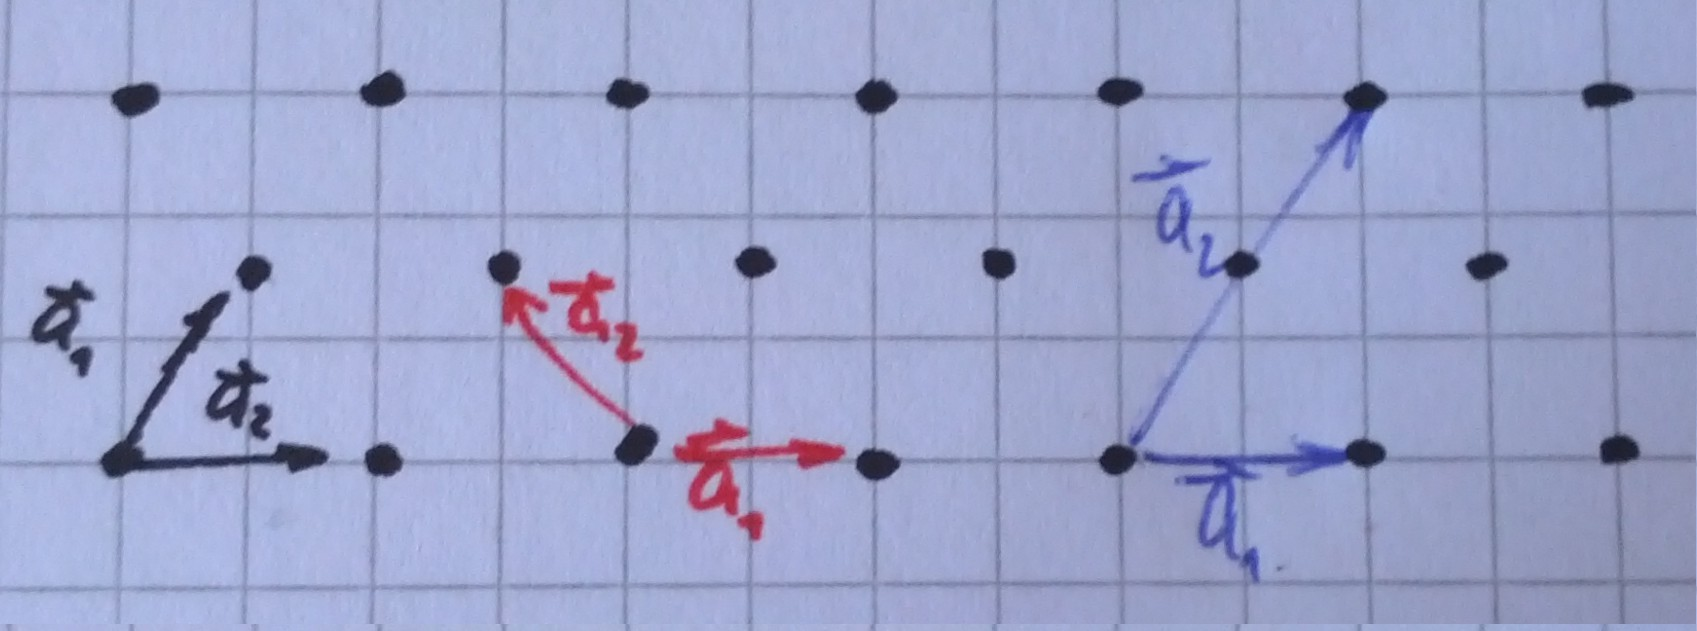
\includegraphics[width=0.6\textwidth]{pics/pic001.jpg}
				%\caption{Vektoren zwischen Gitterpunkten}
			\end{figure}
					
\marginpar {24.10.2013}

			d.h. von den Punkten $\vec{r}$, $\vec{r}\, '$ sieht das 
			Gitter gleich aus wenn gilt
			\begin{center}
			\fbox{$\vec{r}\, ' = \underbrace{\vec{r} + u \vec{a_1} + 
			v \vec{a_2} + w \vec{a_3}}_{\text{\normalfont 
			\emph{Gittertranslation $\vec{T}$}}} ; 
			\; u, v, w \in \mathbb{Z}$}	
			\end{center}		
			Die Wahl von $\vec{a_1}$, $\vec{a_2}$ und $\vec{a_3}$ ist 
			\emph{nicht} eindeutig. Man bezeichnet die Wahl als 
			\emph{primitiv}, wenn durch $\vec{T}$ \emph{alle} 
			gleichartigen Punkte dargestellt werden können.
			Eine \emph{primitive Elementarzelle} hat das kleinste 
			Volumen des aufgespannten Parallelepipels 
			\begin{align*}
				V=\abs{(\vec{a_1} \times \vec{a_2}) \cdot \vec{a_3}}
			\end{align*}
			Die \emph{Wiegner-Seitz-Zelle} ist eine spezielle primitive 
			Elementarzelle. Sie hat folgende Konstruktionsvorschrift
			\begin{figure}[H]
				\centering
				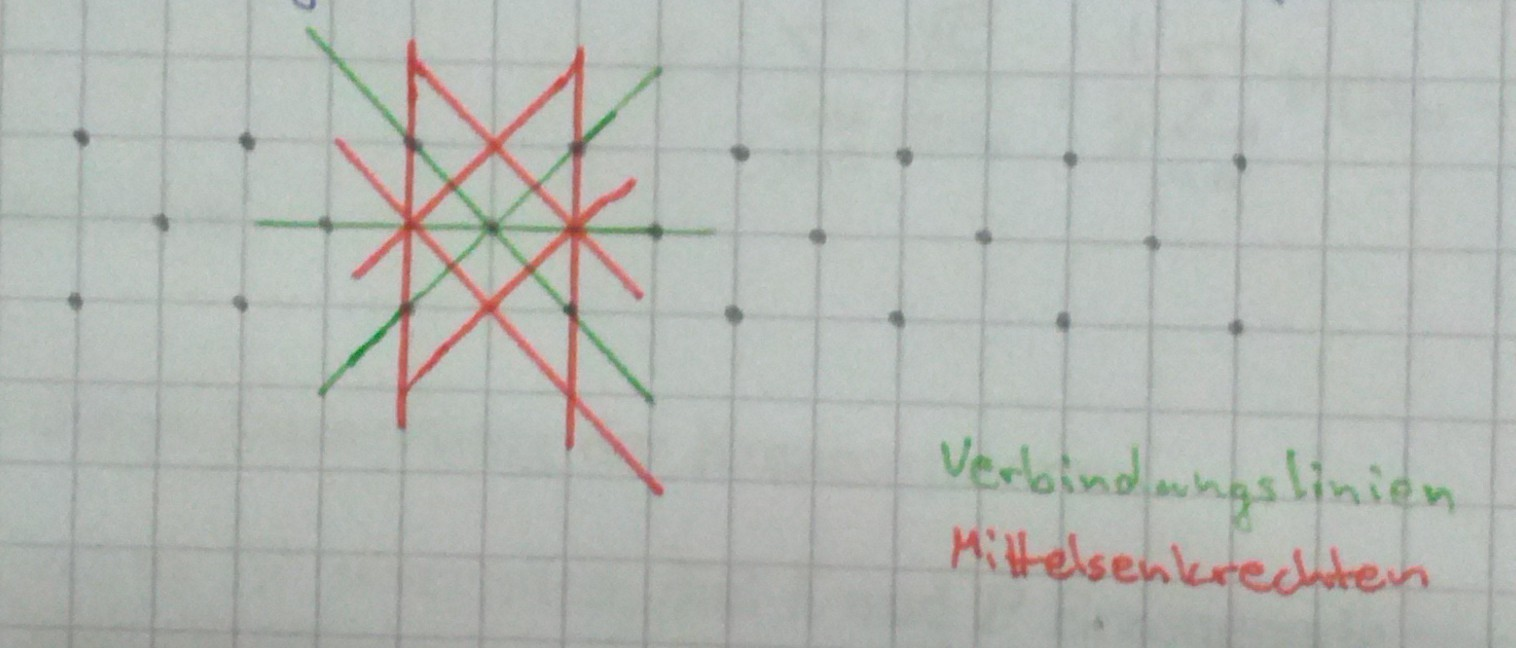
\includegraphics[width=0.6\textwidth]{pics/pic002.jpg}
				%\caption{}
			\end{figure}
			Jeder Gitterpunkt kann mit einer Basis von Atomen besetzt 
			werden.
			\begin{center}
				\fbox{Kristallstruktur = Gitter + Basis}
			\end{center}
			\begin{figure}[H]
					\centering
					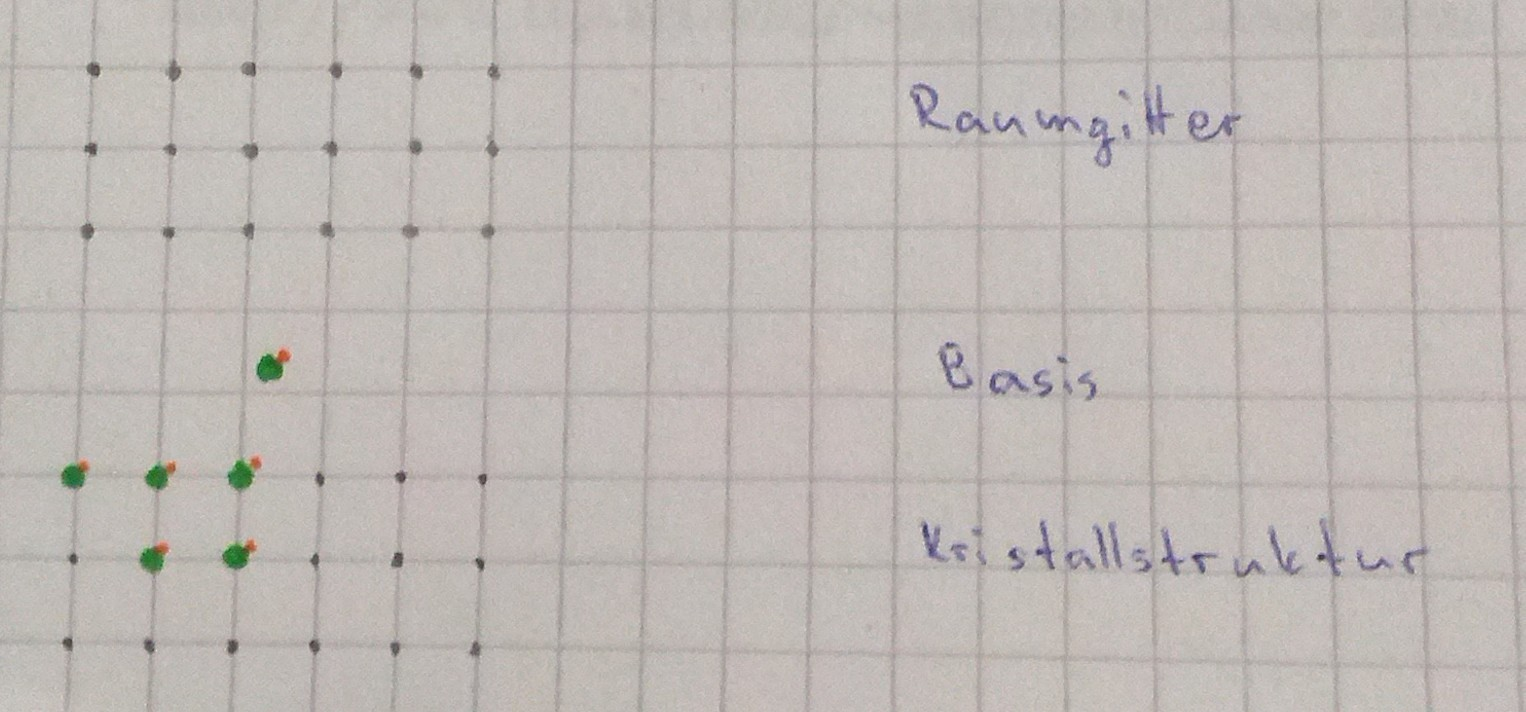
\includegraphics[width=0.6\textwidth]
					{pics/pic003.jpg}
					%\caption{}
			\end{figure}
				Ein Kristall zeichnet sich durch seine \emph{Symmetrien} 
				aus:
			\begin{itemize}
				\item Translationen (s.o.)
				\item Spiegelungen
				\item Drehsymmetrien
			\end{itemize}
			\paragraph*{Definition:} Eine Drehachse, bei der der Kristall nach 
			Drehung um den Winkel $\nicefrac{2\pi}{n}$ 
			($n \in \mathbb{N}$) in sich selbst übergeht, heißt 
			\emph{n-zählige Drehachse}\\
			\paragraph*{Behauptung:} $n=1, 2, 3, 4, 6$; sonst keine Werte 
			möglich\\
			\paragraph*{Beweis:} 
			\begin{figure}[H]
					\centering
					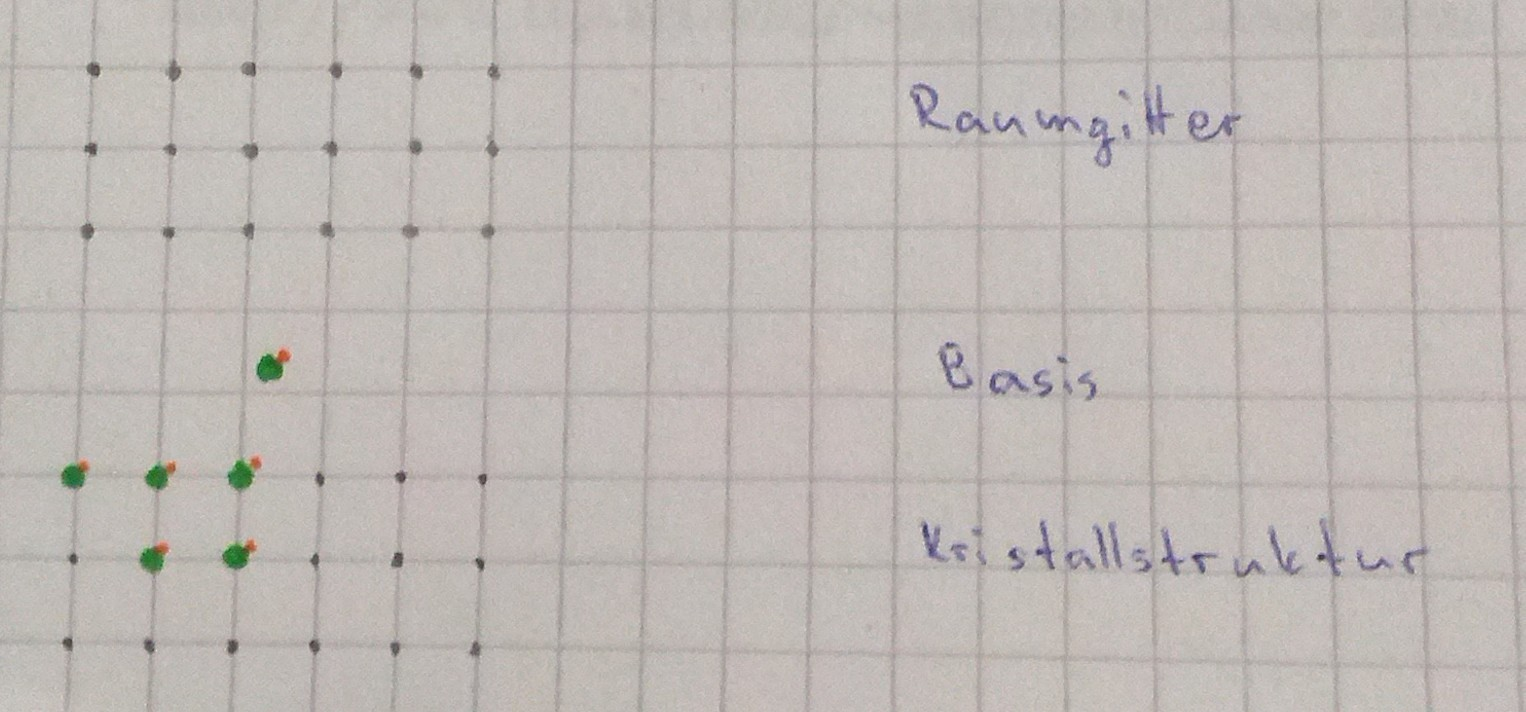
\includegraphics[width=0.6\textwidth]
					{pics/pic003.jpg}
					%\caption{}
			\end{figure}
			\begin{align*}
				&\vec{a}=\left( \begin{smallmatrix} 1 \\ 0 
				\end{smallmatrix}
				\right)	\;\text{ist Translationsvektor}\\
				&\begin{rcases}
					a_+ = \left( \begin{smallmatrix} \cos 
					(\nicefrac{2\pi}{n}) \\ \sin (\nicefrac{2\pi}{n}) 
					\end{smallmatrix} \right)\\
					a_- = \left( \begin{smallmatrix} \cos 
					(\nicefrac{2\pi}{n}) \\ -\sin (\nicefrac{2\pi}{n}) 
					\end{smallmatrix} \right)\\
				\end{rcases}
				\begin{array}{l}
					\text{ist ein blablabla}\\
					\text{aber auch ein blablabla}
				\end{array}
			\end{align*}
			$\Rightarrow$ auch $\vec{a_+}+\vec{a_-}$ ist ein 
			Gittervektor $=a \left( \begin{smallmatrix} \cos 
			(\nicefrac{2\pi}{n})\\ 0 \end{smallmatrix} \right)$. Wenn 
			$\vec{a}$ kleinster Translationsvektor ist, muss gelten
			\begin{align*}
				\vec{a_+}+\vec{a_-} = m \vec{a}; m \in \mathbb{Z}\\
				\Rightarrow \boxed{\underbrace{2\cos 
				(\nicefrac{2\pi}{n})}_{\text{\normalfont Wann ist dies 
				eine ganze Zahl?}} = m}	
			\end{align*}
			\paragraph*{graphisch:}
			\begin{figure}[H]
				\centering
				\begin{minipage}[c]{0.6\textwidth}
					\centering
					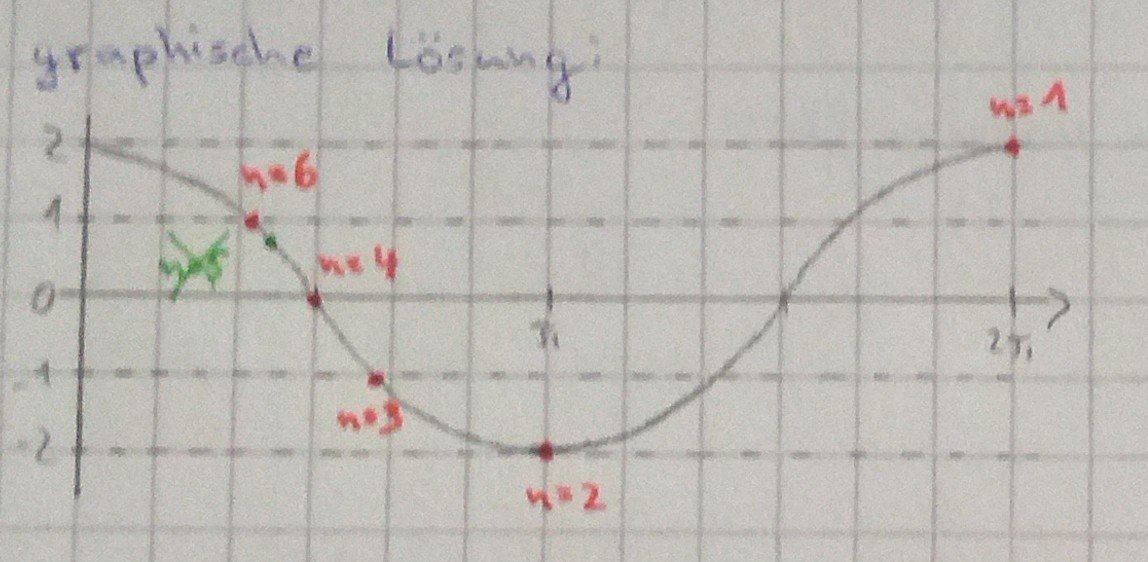
\includegraphics[width=0.9\textwidth]
					{pics/pic005.jpg}
				\end{minipage}	
				\begin{minipage}[c]{0.39\textwidth}
					\centering
					\begin{tabular}{cc}
						\toprule
						$n$ & $2 \cos (\nicefrac{2\pi}{n})$ \\
						\midrule
						1	&	2	\\
						2	&	-2	\\
						3	&	-1	\\
						4	&	0	\\
						5	&	0,61\\
						6	&	1	\\
						7	&	1,25\\
						\vdots & \vdots\\
						\bottomrule
					\end{tabular}
				\end{minipage}	
			\end{figure}
			$\Rightarrow$ $n \in {1, 2, 3, 4, 6}$ q.e.d.\\
			
			In 3D existieren 14 verschiedene Raumgitter, die man als 
			\emph{Bravais-Gitter} bezeichnet. Diese können in sieben 
			verschiedene \emph{Kristallsysteme} 
			eingeordnet werden.\\
			
			BILD POWERPOINTFOLIE\\

\marginpar {29.10.2013}	

			Häuufig möchte man Netzebenen bzw. Netzebenenscharen kennen.
			$\Rightarrow$ Miller'sche Indizes
			
			\paragraph*{Definition:} Gegeben seien die Kristallachsen 
			$\vec{a_1}$, $\vec{a_2}$, $\vec{a_3}$ (nicht unbedingt 
			kartesisch, nich unbedingt primitiv). Die Ebene sei 
			aufgespannt durch die drei Vektoren $n_{1}\vec{a_1}$, 
			$n_{2}\vec{a_2}$, $n_{3}\vec{a_3}$; $n_{1}, n_{2}, n_{3} 
			\in \mathbb{N}$
			\begin{figure}[H]
				\centering
				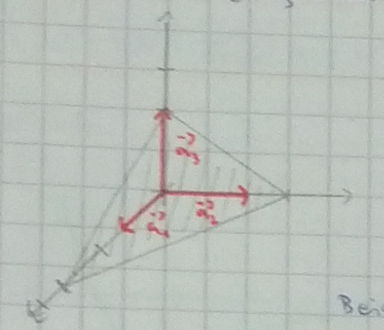
\includegraphics[width=0.6\textwidth]{pics/pic006.jpg}
				%\caption{}
			\end{figure}
			Die (kleinsten) ganzen Zahlen, die sich verhalten wie die 
			Kehrwerte von n1, n2, n3 bilden die Miller'schen Indizes.
			\emph{Beispiel}: $\left( \frac{1}{2}, \frac{1}{3}, 
			\frac{1}{1} \right) \Rightarrow (3,2,6)$. Meist lässt man 
			die Kommata weg, also "`$(326)$"'. Negative Werte werden 
			durch Balken dargestellt, also z.B $(32\overline{6})$. Wird 
			eine Achse nicht geschnitten (ist also der Achsenabschnitt 
			= $\infty$), so ist der zugehörige Miller'sche Index $=0$.
			\paragraph*{Beispiel:} 
				\begin{figure}[H]
					\centering
					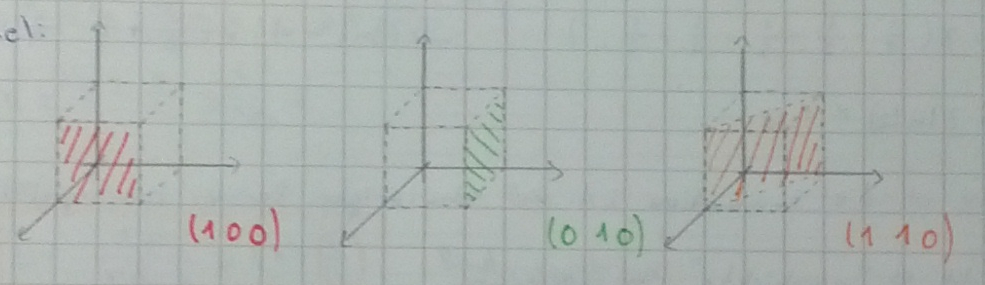
\includegraphics[width=0.6\textwidth]{pics/pic007.jpg}
					%\caption{}
				\end{figure}
			
		\subsubsection{Einfache Kristallstrukturen und ihre Bindung}
			\paragraph*{Natriumchloridstruktur:}
				\subparagraph*{Beispiel:} NaCl, KCl, MnO, KBr, $\ldots$
				\subparagraph*{Bravais-Gitter:} kubisch 
				flächenzentriert (fcc)
				\subparagraph*{Basis:} ein Na und ein Cl (beim NaCl)
				\subparagraph*{Bindung:} ionisch
				Na hat die Elektronenkonfiguration 
				1s$^{2}$2s$^{2}$2p$^{6}$3s$^{1}$ Cl 
				1s$^{2}$2s$^{2}$2p$^{6}$3s$^{2}$3p$^{5}$ $\Rightarrow$ 
				gibt das Na ein Elektron an das Cl ab, so weisen beide 
				abgeschlossene Schalen auf. Es entsteht ein Na$^{+}$ 
				und Cl$^{-}$ Ion, die sich auf Grund der Coulombkraft 
				anziehen\\
				Wir betrachten \emph{$N=N_{A}$} Ionenpaare. Es v die 
				Coulombenergie
				\begin{align*}
					U^{c} = & N \sum_{j, j\neq i} \frac{\pm e^{2}}{4\pi 
					\epsilon_{0} r_{ij}}\\
					& + \text{entspricht Abstoßung Na$^{+}$Na$^{+}$ (i 
					in Na$^{+}$ gewählt)}\\
					& - \text{entspricht Anziehung Na$^{+}$Cl$^{-}$}
				\end{align*}
				Mit der Definition $r_{ij} := p_{ij}r_{0}$, $r_{0}$ ist 
				der Abstand nächster Nachbarn wird hieraus
				\begin{align*}
					U^{c} = \frac{Ne^{2}}{4\pi\epsilon_{0}r_{0}} 
					\underbrace {\sum_{j, j \neq i} 
					\frac{\pm 1}{p_{ij}}}_{\coloneqq -\alpha}
				\end{align*}
				$[\alpha] = 1$, $\alpha > 0$ sonst $U^{c} > 0$
				
				\paragraph*{Beispiel:} (1D Kette)\\
				BILD
				
				$\alpha = 2\left( \frac{1}{1} - \frac{1}{2} + 
				\frac{1}{3} - \frac{1}{4} + \frac{1}{5} \ldots \right)$
				mit $\ln (1+x) =x - \frac{x^{2}}{2} + \frac{x^{3}}{3} - 
				\frac{x^{4}}{4} + \frac{x^{5}}{5} \ldots$\\
				In 3D ist die Summation im Allgemeinen \emph{viel} 
				schwieriger. Die Reihen konvergieren oft schlecht 
				$\Rightarrow${}	"`geschickte"' umgruppierung der 
				Summanden\\
				
				\paragraph*{Beispiel:} (NaCl)\\
				\begin{figure}[H]
					\centering
					\begin{minipage}[c]{0.5\textwidth}
						\centering
						\begin{tabular}{cc}
							\toprule{}
							Ionen		&	Abstand		\\
							\midrule{}
							Na$^{+}$	&	0			\\
							6Cl$^{-}$	&	$r_{0}$		\\
							12Na$^{+}$	&	$\sqrt{2}r_{0}$\\
							8Cl$^{-}$	&	$\sqrt{3}r_{0}$\\
							6Na$^{+}$	&	$\sqrt{4}r_{0}$\\
							\vdots		&	\vdots{}	\\
							\bottomrule
						\end{tabular}
					\end{minipage}	
					\begin{minipage}[c]{0.49\textwidth}
						$\Rightarrow \alpha = \frac{6}{1} - 
						\frac{12}{\sqrt{2}} + \frac{8}{\sqrt{3}} - 
						\frac{6}{\sqrt{4}} = 1,7475$
					\end{minipage}
				\end{figure}
				
				$\sum = 6; -2,48; 2,133; -0,86;$
				
				Es existiert auch eine Abstoßende wechselwirkung auf 
				Grund der überlappenden Elektronenhüllen und des 
				\emph{Pauliverbots}. Dies ist ein quantenmechanischer 
				Effekt. Man setzt \emph{phänomenologisch} an
				\begin{center}
					\fbox{$U_{i}^{B} = +Be^{\nicefrac{r_{ij}}{\rho}}$} 
					Born-Mayer-Potential
				\end{center}	
				$B$ und $\rho$ sind materialspezifische Konstanten. 
				Summation also nur über nächte Nachbarn (NN)
				\begin{align*}
					U^{B} = & N \cdot z \cdot B \cdot 
					e^{\nicefrac{r_{ij}}{\rho}}\\
					& \text{$N$: Zahl der Ionenpaare}\\
					& \text{$z$: Zahl der nächsten Nachbarn, auch 
					"`Koordinationszahl"', z.B. Na$^{+}$ hat $z = 6$}					
				\end{align*}
				Die gesamte Energie ist 
				\begin{align*}
					U = & U^{C} + U^{B}\\
					\Rightarrow U = & -N \left( 
					\frac{e^{2}}{4\pi\epsilon_{0}} \alpha - z \cdot B 
					e^{ \nicefrac{ r_{0} }{ \rho} } \right)
				\end{align*}
				\paragraph*{graphisch:}
				BILD\\
				
				Gleichgewichtslage bei $\frac{dU}{dr_{0}}=0$
				\begin{align*}
					\Rightarrow & 0 = -N \left( \frac{-e^{2}}{4\pi{}
					\epsilon_{0} r_{0}^{2}}\alpha - zB(1/\rho)e^{
					\frac{-r_{0}}{\rho}} \right) \\
					\Rightarrow & z B e^{\nicefrac{r_{0}}{\rho}} = 
					\frac{\rho}{r_{0}} \frac{e^{2}}{4\pi\epsilon_{0} 
					r_{0}} \alpha
				\end{align*}
				Einsetzen:
				\begin{center}
					$\Rightarrow$ \fbox{$U = \frac{-Ne^{2}}{4\pi{}
					\epsilon_{0}r_{0}}\alpha \Bigg( 1 - \underbrace{
					\frac{\rho}{r_{0}}}_{\ll 1}\Bigg)$} Bindungsenergie
				\end{center}
				Die Bindungsenergie pro Ionenpaar N ist 
				\begin{align*}
					E_{B} \coloneqq \frac{U}{N}
				\end{align*}
				\paragraph*{Beispiel:} (NaCl)
				\begin{center}
					$\begin{rcases}
						r_{0} = 0,28nm\\
						\rho = 0,03nm
				\end{rcases}$
				$E_{B} = 8,23\text{eV (starke Bindung)}$\\		
				\end{center}	
			\paragraph*{Cäsiumchlorid:}
				\subparagraph*{Beispiel:} CsCl, CnPd, AlNi, AgMg, 
				$\ldots$
				\subparagraph*{Bravais-Gitter:} einfach kubisch
				\subparagraph*{Basis:} ein Cs und ein Cl
				\subparagraph*{Bindung:} ionisch; Cs hat 
				Elektronenkonfiguration 
				1s$^{2}$2s$^{2}$2p$^{6}$3s$^{2}$3p$^{5}$3d$^{10}$
				4s$^{2}$4p$^{6}$4d$^{10}$5s$^{2}$5p$^{6}$6s$^{1}$,	Cl 
				hat Elektronenkonfiguration 1s$^{2}$2s$^{2}$2p$^{6}$
				3s$^{2}$3p$^{5}$ $\Rightarrow$ analog zum NaCl
				
\marginpar {31.10.2013}	
				
			\paragraph*{Hexagonal dichteste Kugelpackung:}
				\subparagraph*{Beispiel:} He, Zn, Co, Opale, $ßldots$
				\subparagraph*{Bravais-Gitter:} es existieren zwei 
				Möglichkeiten dichtester Kugelpackung ($\approx 74\%$)
				\begin{enumerate}
					\item	Hexagonal dichteste Packung (hcp)\\
							BILD\\
							Schichtfolge ABABAB$\ldots${}\\ 
							$\Rightarrow${}
							hexagonal primitive Elementarzelle mit Basis
							aus zwei Atomen
					\item	Flächenzentrierte dichteste Packung (fcc)\\
							BILD\\
							Schichtfolge ABCABCABC$\ldots${}\\ 
							$\Rightarrow${}
							fcc Elementarzelle mit einatomiger Basis
				\end{enumerate}

				\subparagraph*{Bindung:} van der Waals Wechselwirkung
				Edelgasatome (z.B. He, Ne) besitzen bereits 
				abgeschlossene Schalen. Die
				Bindungsenergie durch die Wechselwirkung ist sehr 
				klein, z.B. bei Neon $E_{B}=0,02\nicefrac{eV}{Atom}$\\
				\subparagraph*{Einfaches Modell:}
				BILD\\
				\subparagraph*{Näherungen:} $M \gg m , r \gg 
				\abs{x_{1}}, \abs{x_{2}}$ $\Rightarrow$ 
				quantenmechanische Grundzustandsenergie $=
				\frac{\hbar}{2} \left( 2 \frac{D}{m} - \frac{2}{8} 
				\left( \frac{2e^{2}m}{4\pi\epsilon_{0}r^{3}} \right) 
				\right) \propto \frac{1}{r^{6}}$ $\Rightarrow \hbar = 0 
				\Rightarrow$ keine Wechselwirkung
			\paragraph*{Diamantstruktur:}
				\subparagraph*{Beispiele:} C, Si, Ge, $\ldots${}
				\subparagraph*{Bravais-Gitter:} fcc
				\subparagraph*{Basis:} zwei identisch Atome bei 
				$(0,0,0)$ und ($\nicefrac{1}{4}$, $\nicefrac{1}{4}$, 
				$\nicefrac{1}{4}$). Die Raumausfüllung ist sehr 
				schlecht mit $34\%$ (vgl. $74\%$ bei hcp)
				\subparagraph*{Bindung:} kovalent; die 
				Elektronenkonfiguration des Kohlenstoffatoms ist 
				1s$^{2}$2s$^{2}$2p$^{2}$, d.h. es fehlen 4 Elektronen 
				um die Schale zu schließen. $\Rightarrow$ tetraedrische 
				Bindung mit vier nächsten Nachbarn.\\Typische 
				Bindungsenergien Kohlenstoff $E_{B} = 3,6$eV Silizium 
				$E_{B} = 1,8$eV. Zwischen der \emph{kovalenten} und der
				\emph{ionischen} Bindung gibt es einen kontinuierlichen 
				Übergang.\\Elemente der Hauptgruppen	\textsc{III}, 
				\textsc{IV} und \textsc{V} tendieren zur kovalenten 
				Bindung (z.B GaAs), Elemente mit fast abgeschlossenen 
				Schalen zur ionischen Bindung. Bei der 
				\emph{metallischen Bindung} werden die Elektronen 
				völlig delokalisiert, d.h. feste Ionenrümpfe und ein 
				"`Gas"' freier Elektronen ($\Rightarrow$ gute 
				Leitfähigkeit)			
			\paragraph*{Kubische Zinksulfidstruktur:}
				\subparagraph*{Beispiel:} CdS, ZnS, SiC, $\ldots$
				\subparagraph*{Bravais-Gitter:} fcc
				\subparagraph*{Basis:} ein Zn und ein S $\Rightarrow$ 
				keine Inversionssymmetrie ($\vec{r} \; 
				\cancel{\rightarrow} -\vec{r}$)	
	
	\subsection{Das reziproke Gitter und Methoden der Strukurbestimmung}
		\paragraph{Beugung von Röntgenstrahlung am Kristall:}
			BILD
			\subparagraph{Behauptung:} Die Beugungsamplitude ist 
			proportional zur Fouriertransformierten der Elektronendichte
			\subparagraph{Beweis:} Voraussetzungen:
				\begin{enumerate}
					\item	elastische Beugung $\Leftrightarrow$ 
					Energieerhaltung $\Leftrightarrow \abs{k} = 
					\abs{k'}$
					\item	einmalige Streuung im Kristall
					\item	lokale Amplitude ist proportional zur 
					Elektronendichte $\rho (\vec{r})$
				\end{enumerate}
		
		BILD
		
		\begin{align*}
			\Delta = \cos (\phi) \cdot \abs{\vec{r}} \\
			\Delta \phi = \frac{2\pi}{\lambda} entpsricht \text{Phasenverschiebung} \\
			\Rightarrow \Delta \phi = \frac{2\pi}{\lambda} \cos (\phi) abs{\vec{r}} = \abs{\vec{k}} \cdot \abs{\vec{r}} \cdot \cos (\phi) = \vec{k} \cdot \vec{r} \\
			\Delta ' = \sin \alpha \cdot \abs{vec{r}} = \sin (\phi ' - 90°) \cdot XXXX = -\cos (\phi ') \cdot \abs{vec{r}} \\
			\Delta \phi_{ges} = (\vec{k} - \vec{k'}) \cdot \vec{r} =: \Delta \vec{k} \cdot \vec{r}
		\end{align*}
		summiere über alle Orte $\vec{r}$ $\rightarrow$ Beugungsamplitude
		\begin{align*}
			A(\Delta\vec{k}) \propto \int_{-\inf}^{+\inf} \rho (\vec{r}) e^{-i\Delta\vec{k}\cdot\vec{r}} d^{3}x
		\end{align*}		
		KASTEN DRUM
		oder umgekehrt
		\begin{align*}
			\rho (\vec{r}) \propto \int_{-\inf}^{+\inf} A(\Delta\vec{k}) e^{+i\Delta\vec{k}\cdot\vec{r}} d^{3}x
		\end{align*}
		KASTEN DRUM
		\begin{itemize}
		\item Im Allgemeinen werden jedoch Intensitäten gemessen (Betrag des Poyntingvektors); Messung $\Rightarrow \abs{A}^{2} entspricht \text{Intensität} druchgestrichernerdoppelpfeil A \in \mathbb{C}$
		$\Rightarrow \rho (\vec{r})$ kann nicht ohne weiteres bestimmt werden\\
		\item A ist Funktion von 
		
			\item	Richtungsänderung
			\item	Wellenlänge
		\end{itemize}
		
		Die Ladungsdichte $\rho (\vec{r})$ ist eine Gitterfunktion und bezüglich Translationen von Gittervektoren invariant, d.h.
		$\rho (\vec{r}) = \rho (\vec{r}+\vec{T})$ mit $\vec{T} = u\vec{a_{1}} + v\vec{a_{2}} + w\vec{a_{3}}$, $u, v, w \in \mathbb{Z}$
		\begin{align*}
			A(\Delta\vec{k}) \propto \int_{-inf}^{+inf} \rho (\vec{r}) e^{irgendwasvonoben} d^{3}x\\
			=\int_{-inf}^{+inf} \rho (\vec{r}-\vec{T}) e^{sdafjadslk} d^{3}x \\
			\int_{-inf}^{+inf} \rho (\vec{r}) e^{-i\Delta\vec{k}(\vec{r}-\vec{T})} d^{3}x \\
			=
 		\end{align*}
		 
		
		
		
		
		
		
		
		
		
		
		
		
\end{document}
